%% Porocilo iz vaj pri reologiji
%% Junij 2015
%% Ivan Pribec, Jasmina Sedmak, Filip Strniša

\documentclass{article}

\usepackage{color}
\usepackage{epsfig,graphics}
\usepackage{amsmath}

\usepackage[utf8]{inputenc}
\usepackage[protrusion=true,
            expansion=true
           ]{microtype}

\usepackage[slovene]{babel}
\usepackage{graphicx} 
\usepackage{caption}          % Needed for including graphics.
\usepackage{url}                % Facility for activating URLs.

\usepackage[a4paper,margin=2.4cm]{geometry}

\usepackage{tabularx}
\newcolumntype{Y}{>{\centering\arraybackslash}X}

\usepackage{subcaption}
\usepackage{wrapfig}
\usepackage{sidecap}
\usepackage{breakurl}
\usepackage{booktabs}
\setlength{\heavyrulewidth}{1.1pt}
\setlength{\abovetopsep}{1pt}

\renewcommand{\refname}{Literatura} 

%%%%%%%%%%%%%%%%%%%%%%%%%%%%%%%%%%%%%%%%%%%%%%%%%%%%%%%%%%%%%%%%%%%%%%
%% Start of the document.
%%%%%%%%%%%%%%%%%%%%%%%%%%%%%%%%%%%%%%%%%%%%%%%%%%%%%%%%%%%%%%%%%%%%%%

\begin{document}

\author{Ivan Pribec, Jasmina Sedmak, Filip Strniša\\
Fakulteta za kemijo in kemijsko tehnologijo, Univerza v Ljubljani}
\date{Ljubljana, 27.06.2015}
\title{Poročilo iz vaj pri predmetu \textit{Reologija kompleksnih tekočin}\\
Reološke lastnosti gelov}
\maketitle


\section{Namen vaje}
Cilj tokratnih vaj iz reologije je bila seznanitev z uporabo rotacijskega viskozimetra z nastavljivo strižno deformacijo in spoznavanje različnih merilnih tehnik pri nedestruktivnih in destruktivnih strižnih pogojih. Poseben poudarek je bil na merilnih tehnikah za viskoelastične tekočine (oscilatorni testi in testi lezenja in obnove). Pridobljene rezultate smo tudi interpretirali s pomočjo različnih reoloških modelov in risanjem reoloških grafov. Testirane snovi so bile vodne raztopine polisaharidov gelana in ksantana.

\section{Teoretične osnove in metode dela}

Pojem \textbf{gel} se uporablja za opisovanje želatini podobne, bolj ali manj rigidne snovi, ki se tvori s tem, ko se koloidni delčki med seboj povežejo v tridimenzionalno mrežo ali pa pri premreženju polimernih molekul. Čeprav lahko večino mase gela predstavlja tekočina (npr. voda) je premreženje tisto, ki daje gelu svoje trdno strukturo. Veliko gelov izkazuje tiksotropijo, saj se ob agitaciji njihova struktura podre in lahko stečejo. Prav tako izkazujejo mejno napetost in viskoelastične lasnosti. Pri vaji smo uporabili dva polisaharidska gela na osnovi ksantana in gelana:
\begin{itemize}
\item KSANTAN je naravni polisaharid, ki nastane pri fermentaciji sladkorjev s z bakterijo \textit{Xanthomonas campestris}. Uporablja se ga kot regulator viskoznosti, gostilo, gelirno sredsvo in stabilizator emulzij v prehranski (E415; pudingi, solatne polivke, sladoled in peka kruha) in kozmetični industriji (kreme, losjoni, zobna pasta).
 \item GELLAN je anionski polisaharid, ki ga proizvajajo bakterije \textit{Sphingomonas elodea}. Uporablja se ga kot alternativno gelirno sredstvo agarju v mikrobiologiji in pri gojenju rastlinskih celičnih kultur. Uporabo pa ima tudi v prehranski (E418), kozmetični in farmacevtski industriji kot gostilo, emulgator, stabilizator in gelirno sredstvo.
\end{itemize}

Iz že pripravljenega gela dane koncentracije polisaharida smo vzeli izračunano količino in jo raztopili v vodi, segreli do vrenja in prekuhali za 10 minut. Tako smo pripravili 0,5, 0,7 in 1,0 \% raztopine gelana in 1,0 \% raztopino ksantana. Kljub nizkim koncentracijam imajo take raztopine šibkogelski značaj. Ob stresanju oz. izpostavljenosti strigu se taka struktura podre in snov steče.

Najpopularnejši instrument za reološko karakterizacijo snovi je zagotovo \textbf{rotacijski viskozimeter} kot je prikazan na sliki \ref{fig:viskozimeter}. Deluje na principu merjenja navora, ki je potreben, da vrtimo senzorski sistem v stiku s tekočino. Na podlagi vrtilne hitrosti in geometrije senzorskega sistema lahko izračunamo viskoznost tekočine. Takemu reometru pravimo tudi reometer z nastavljivo strižno hitrostjo. Modernejši tip reometra, je rotacijski viskozimeter z nastavljivo strižno deformacijo. V takem reometru je nastavljena vrednost navora, odpor vzorca proti nastavljeni strižni napetosti pa povzroči odmik rotorja. Hitrost rotorja in pozicijo se izmeri z digitalnim optičnim kodirnikom. Sistem mora biti zračno uležajen. Reometer z nastavljivo strižno napetostjo omogoča izvedbo zahtevnejših merilnih tehnik kot so testi lezenja in obnove ter oscilatorni testi.

\begin{figure}
   \centering
   \begin{subfigure}[b]{0.3\textwidth}
       \includegraphics[width=\textwidth]{rheometer2.jpg}
   \end{subfigure}
   \qquad %add desired spacing between images, e. g. ~, \quad, \qquad, \hfill etc. 
     %(or a blank line to force the subfigure onto a new line)
   \begin{subfigure}[b]{0.4\textwidth}
       \includegraphics[width=\textwidth]{plosca_plosca.jpg}
   \end{subfigure}
   
   \caption{Rotacijski viskozimeter in senzorski sistem dveh vzporednih plošč podoben tistemu, ki smo ga uporabili med izvedbo vaje. Vir: \burl{http://www.usm.flaneyassociates.com/ResearchFacilities/Rheology.htm}}
   \label{fig:viskozimeter}
\end{figure}

Za reološko karakterizacijo snovi se na rotacijskem viskozimetru poslužujemo različnih merilnih tehnik, pri katerih vzorce izpostavimo statičnim ali dinamičnim strižnim pogojem in sledimo obnašanju materiala preko količin kot so navidezna viskoznost $\eta$, strižna deformacija $\gamma$, strižna hitrost $\dot{\gamma}$, strižna napetost $\tau$, modul akumulacije energije $G^{'}$, modul energetskih izgub $G^{''}$, faktor dušenja $\delta$, kompleksni modul $G^*$ in voljnost $J$. Med vajo smo izmerili naslednje odvisnosti oz. napravili napisane teste (več o posamezni metodi je napisano v poglavju Meritve in rezultati):
\begin{enumerate}
\item Tokovna odvisnost (trikotna metoda)
\item Temperaturna odvisnost
\item Amplitudna odvisnost (oscilatorni test)
\item Frekvenčna odvisnost (oscilatorni test)
\item Test lezenja in obnove
\item Ponavljajoči test lezenja in obnove
\end{enumerate}

Po izvedbi reoloških meritev se pogosto soočamo s problemom, da moramo izmerjenim eksperimentalnim točkam poiskati modelno funkcijo, ki te točke najbolje opiše. S pomočjo modelnih funkcij nato lažje primerjamo vpliv preučevanih spremenljivk (npr. koncentracije, temperature) na dano snov. Reološke modelne funkcije so v večini nelinearne, kar zahteva prav posebno skrb. Imamo torej \textbf{optimizacijski problem}, ki ga rešujemo s pomočjo minimizacije vsote kvadratov razlik med modelnimi in izmerjenimi vrednostmi
\begin{equation}
S = \sum\limits^N_i \big(y^\mathrm{meritev}_i-y^\mathrm{model}_i(\mathrm{\textbf{v}})\big)^2
\end{equation}
kjer $y^\mathrm{meritev}_i$ predstavlja izmerjene vrednosti, $y^\mathrm{model}_i(\mathrm{\textbf{v}})$ izračunane vrednosti, $\mathrm{\textbf{v}}$ je vektor parametrov, ki nastopajo v modelni funkciji in $N$ število eksperimentalnih točk. Reševanja takega problema se lotimo numerično s pomočjo izdelanih programov kot so Excel (orodje \textit{Solver}) in Matlab (funkcija \texttt{lsqnonlin}), ali pa izdelamo svoj program na osnovi jezika Python in različnih namenskih knjižnic (\texttt{scipy.optimize}, \texttt{lmfit}).

%Pri metodi merjenja frekvenčne in tokovne odvisnosti je bila nastavljiva deformacija 1 \%. 
%Pri amplitudni, frekvenčni in tokovni odvisnosti smo najprej merili 1 \% ksantan prvič pri 20 $^\circ$C, drugič pri 30 $^\circ$C. Nato pa še 1 \% gellan, 0,7 \% gellan ter 0,5 \% gellan pri 20 $^\circ$C.
%
%Pri testu lezenja in obnove smo vzorce pomerili pri 20 $^\circ$C. Testirali smo 1 \% ksantan (kjer je bila strižna napetost 0,1 Pa), 1 \% gellan (strižna napetost – 0,3 Pa) ter 0,7 \% gellan.
%
%Metodo temperaturne odvisnosti smo pomerili v temperaturnem območju od 15 $^\circ$C do 50 $^\circ$C ter obratno od 50 $^\circ$C do 15 $^\circ$C z 1 \% gellanom.

\newpage
\section{Meritve in rezultati}

\subsection{Tokovna odvisnost}
Na viskozimetru smo opravili meritve strižne napetosti pri različnih strižnih hitrostih. Aparat je izračunal tudi viskoznost pri danih strižnih hitrostih. Nato smo preverili, kako rezultati pašejo v potenčni model (enačba (\ref{eq:powerm})) in Crossov model (enačba (\ref{eq:Crossm})).

\begin{equation} \label{eq:powerm}
\tau^n = {\tau_0}^n + \Big(\eta_\infty\frac{d\gamma}{dt}\Big)^n
\end{equation}

\begin{equation} \label{eq:Crossm}
\frac{\eta - \eta_{\infty}}{\eta_0 - \eta_{\infty}} = \frac{1}{1 + \Big(K_1\frac{d\gamma}{dt}\Big)^m}
\end{equation}

\subsubsection{Crossov model}

\begin{figure}
	\centering
	\begin{subfigure}[b]{0.4\textwidth}
	       \includegraphics[width=\textwidth]{cross_ksan1.eps}
	   \end{subfigure}
	   % \quad
	   \begin{subfigure}[b]{0.4\textwidth}
	       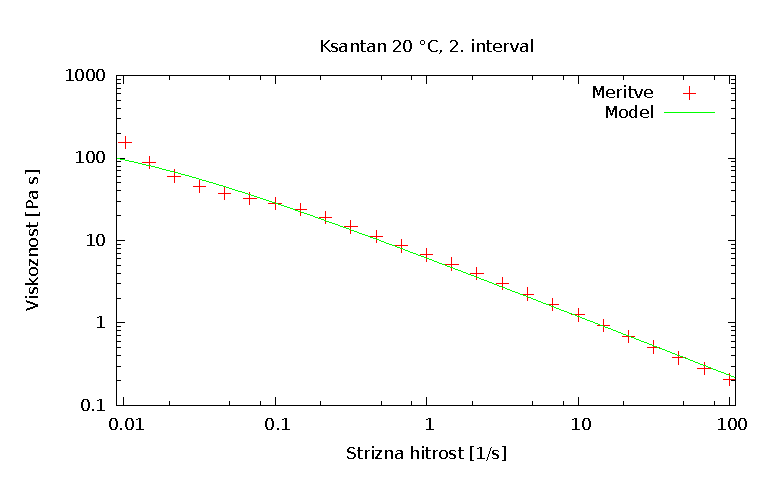
\includegraphics[width=\textwidth]{cross_ksan2.eps}
	   \end{subfigure}
	\caption{Meritve za 1 \% Ksantan pri 20 $^\circ$C. 1. interval: $K_1 = 138,5 s; m = 0,858; \eta_0 = 731,4 Pa s; \eta_\infty = 0,0345 Pa s$. 2. interval: $K_1 = 138,5 s; m = 0,717; \eta_0 = 215,8 Pa s; \eta_\infty = 0 Pa s$.}
	\label{fig:cross_xan1}
\end{figure}

\begin{figure}
	\centering
	\begin{subfigure}[b]{0.4\textwidth}
	       \includegraphics[width=\textwidth]{cross_ksan3.eps}
	   \end{subfigure}
	   % \quad
	   \begin{subfigure}[b]{0.4\textwidth}
	       \includegraphics[width=\textwidth]{cross_ksan4.eps}
	   \end{subfigure}
	\caption{Meritve za 1 \% Ksantan pri 30 $^\circ$C. 1. interval: $K_1 = 116,9 s; m = 0,793; \eta_0 = 348,5 Pa s; \eta_\infty = 0 Pa s$. 2. interval: $K_1 = 96,1 s; m = 0,760; \eta_0 = 231,6 Pa s; \eta_\infty = 0 Pa s$.}
	\label{fig:cross_xan2}
\end{figure}

\begin{figure}
	\centering
	\begin{subfigure}[b]{0.4\textwidth}
	       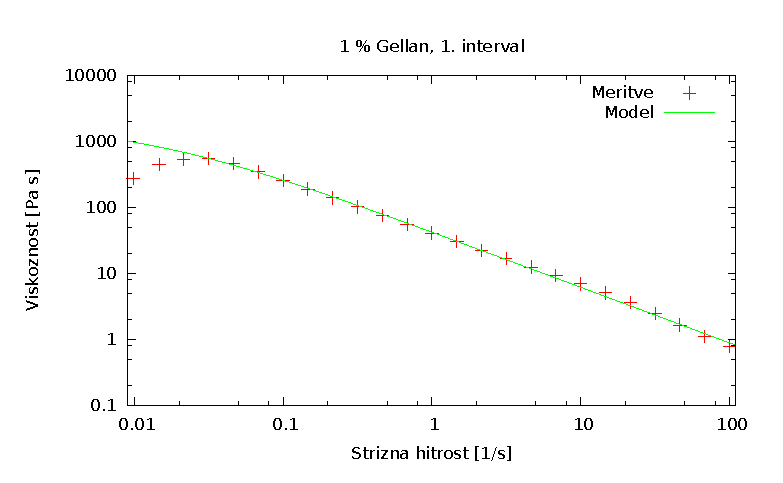
\includegraphics[width=\textwidth]{cross_gel1.eps}
	   \end{subfigure}
	   % \quad
	   \begin{subfigure}[b]{0.4\textwidth}
	       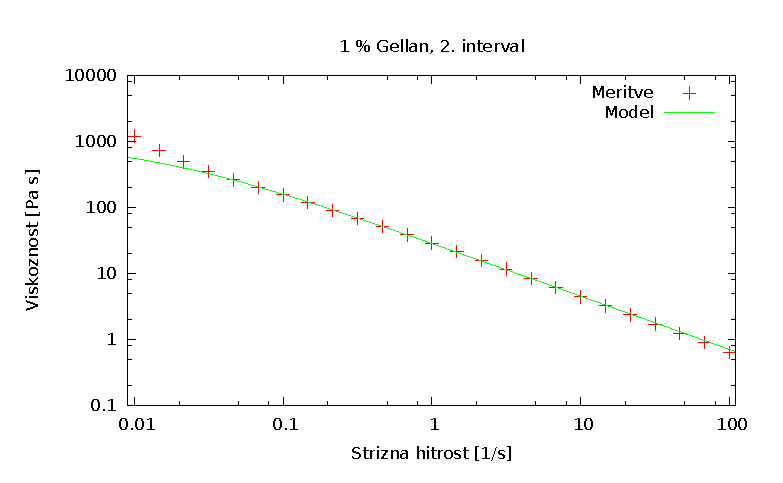
\includegraphics[width=\textwidth]{cross_gel2.eps}
	   \end{subfigure}
	\caption{Meritve za 1 \% Gellan pri 20 $^\circ$C. 1. interval: $K_1 = 83,54 s; m = 0,844; \eta_0 = 1814 Pa s; \eta_\infty = 0 Pa s$. 2. interval: $K_1 = 80,87 s; m = 0,809; \eta_0 = 1022 Pa s; \eta_\infty = 0 Pa s$.}
	\label{fig:cross_gel1}
\end{figure}

\begin{figure}
	\centering
	\begin{subfigure}[b]{0.4\textwidth}
	       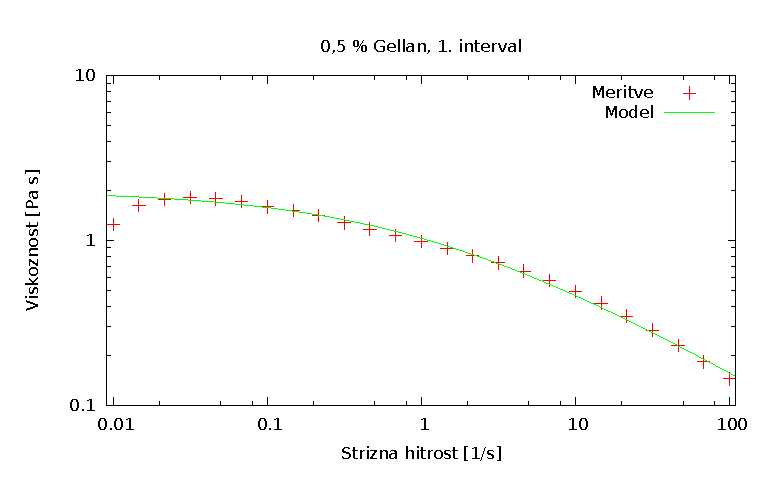
\includegraphics[width=\textwidth]{cross_gel3.eps}
	   \end{subfigure}
	   % \quad
	   \begin{subfigure}[b]{0.4\textwidth}
	       \includegraphics[width=\textwidth]{cross_gel4.eps}
	   \end{subfigure}
	\caption{Meritve za 0,5 \% Gellan pri 20 $^\circ$C. 1. interval: $K_1 = 0,902 s; m = 0,548; \eta_0 = 2,007 Pa s; \eta_\infty = 0 Pa s$. 2. interval: $K_1 = 0,212 s; m = 0,662; \eta_0 = 1,277 Pa s; \eta_\infty = 0 Pa s$.}
	\label{fig:cross_gel2}
\end{figure}

\subsubsection{Potenčni model}

\begin{figure}
	\centering
	\begin{subfigure}[b]{0.4\textwidth}
	       \includegraphics[width=\textwidth]{tok_ksan1.eps}
	   \end{subfigure}
	   % \quad
	   \begin{subfigure}[b]{0.4\textwidth}
	       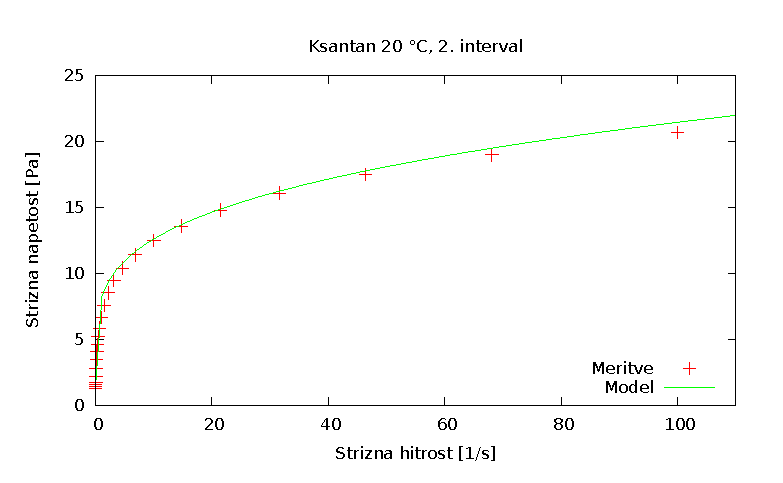
\includegraphics[width=\textwidth]{tok_ksan2.eps}
	   \end{subfigure}
	\caption{Meritve za 1 \% Ksantan pri 20 $^\circ$C. 1. interval: $n = 0,107; \tau_0 = 2,414 Pa; \eta_\infty = 1,63*10^{-7} Pa s$. 2. interval: $n = 0,108; \tau_0 = 1,422 Pa; \eta_\infty = 6,15*10^{-7} Pa s$.}
	\label{fig:tok_ksan1}
\end{figure}

\begin{figure}
	\centering
	\begin{subfigure}[b]{0.4\textwidth}
	       \includegraphics[width=\textwidth]{tok_ksan3.eps}
	   \end{subfigure}
	   % \quad
	   \begin{subfigure}[b]{0.4\textwidth}
	       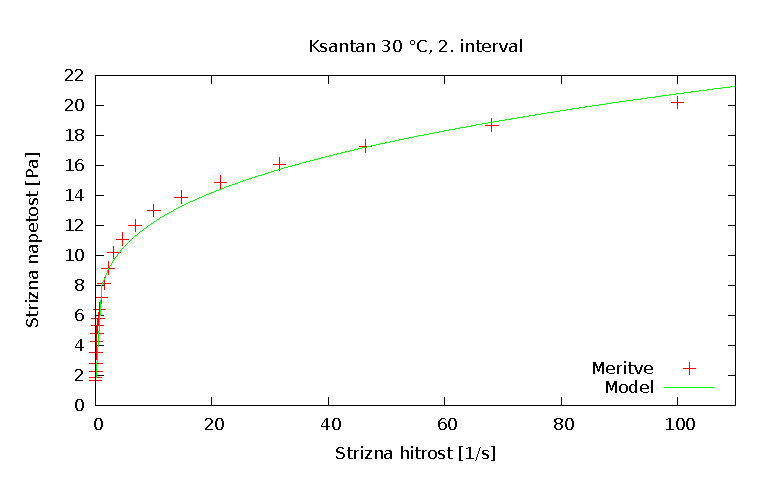
\includegraphics[width=\textwidth]{tok_ksan4.eps}
	   \end{subfigure}
	\caption{Meritve za 1 \% Ksantan pri 30 $^\circ$C. 1. interval: $n = 0,107; \tau_0 = 1,397 Pa; \eta_\infty = 5,26*10^{-7} Pa s$. 2. interval: $n = 0,107; \tau_0 = 1,351 Pa; \eta_\infty = 5,26*10^{-7} Pa s$.}
	\label{fig:tok_ksan2}
\end{figure}

\begin{figure}
	\centering
	\begin{subfigure}[b]{0.4\textwidth}
	       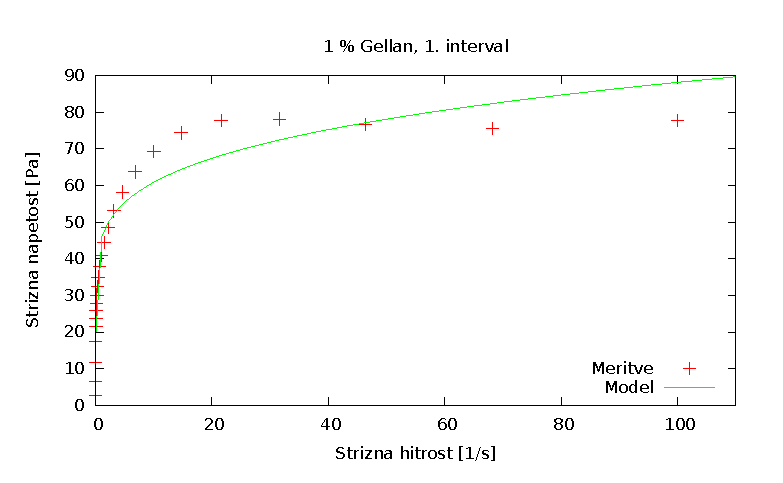
\includegraphics[width=\textwidth]{tok_gel1.eps}
	   \end{subfigure}
	   % \quad
	   \begin{subfigure}[b]{0.4\textwidth}
	       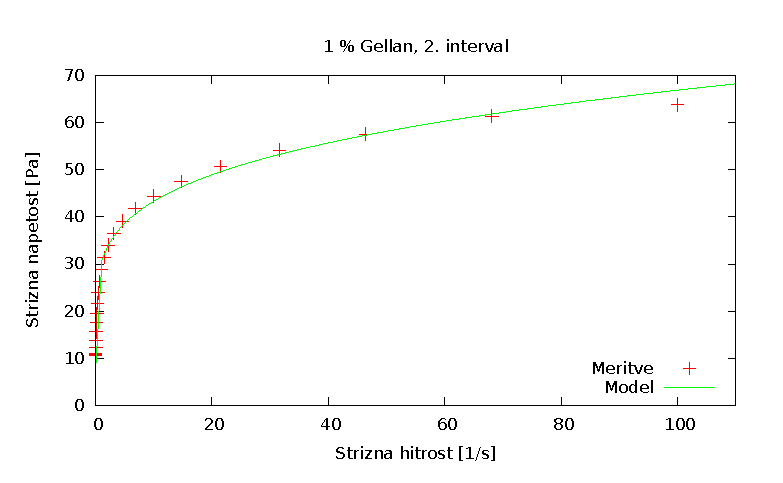
\includegraphics[width=\textwidth]{tok_gel2.eps}
	   \end{subfigure}
	\caption{Meritve za 1 \% Gellan pri 20 $^\circ$C. 1. interval: $n = 0,125; \tau_0 = 17,84 Pa; \eta_\infty = 9,81*10^{-7} Pa s$. 2. interval: $n = 0,105; \tau_0 = 7,270 Pa; \eta_\infty = 2,06*10^{-7} Pa s$.}
	\label{fig:tok_gel1}
\end{figure}

\begin{figure}
	\centering
	\begin{subfigure}[b]{0.4\textwidth}
	       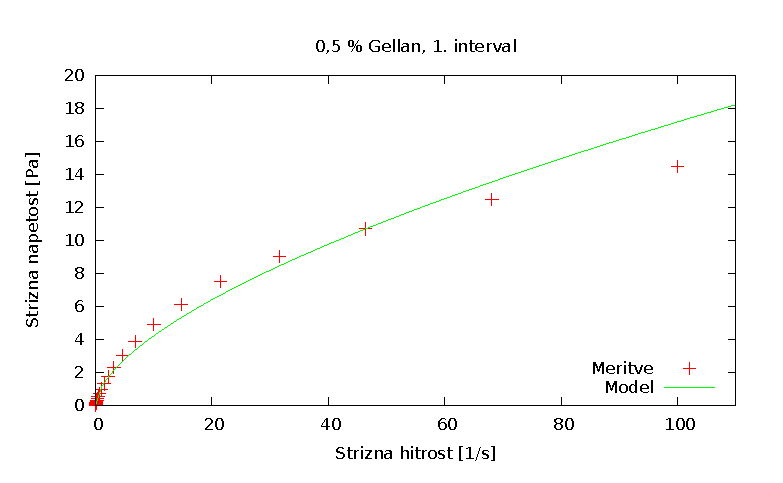
\includegraphics[width=\textwidth]{tok_gel3.eps}
	   \end{subfigure}
	   % \quad
	   \begin{subfigure}[b]{0.4\textwidth}
	       \includegraphics[width=\textwidth]{tok_gel4.eps}
	   \end{subfigure}
	\caption{Meritve za 0,5 \% Gellan pri 20 $^\circ$C. 1. interval: $n = 0,0396; \tau_0 = 4,0*10^{-10} Pa; \eta_\infty = 1,03*10^{-6} Pa s$. 2. interval: $n = 0,0396; \tau_0 = 3,97*10^{-10} Pa; \eta_\infty = 1,05*10^{-6} Pa s$.}
	\label{fig:tok_gel2}
\end{figure}

\subsection{Temperaturna odvisnost}
Na reometru smo merili viskoznost 1 \% Gellana na temperaturnem intervalu 15 - 50 $^\circ$C pri konstantni strižni hitrosti 50 $s^{-1}$. Temperaturo smo spreminjali v obe smeri - torej smo jo zviševali in zniževali.

\begin{figure}
  \centering
  \includegraphics[width=\linewidth]{T_odv.png}
  \caption{Odvisnost viskoznosti $\eta$ 1 \% Gellana od temperature $T$. Zgornja krivulja predstavlja meritve med segrevanjem, spodnja pa med ohlajanjem.}
  \label{fig:temp}
\end{figure}


\subsection{Amplitudna odvisnost}

Območje linearnega viskoelastičnega odziva smo določali z amplitudnim testom, kjer povečujemo amplitudo strižne deformacije pri konstantni frekvenci oscilacije. Kritično vrednost $\gamma_\mathrm{krit}$ smo določali na ta način, da smo eksperimentalnim podatkom prilagodili nasledenjo funkcijo
\begin{equation} \label{eq:ampl}
G^* = G^*_0\frac{1+b\gamma^n}{1+a\gamma^n}
\end{equation}
in izračunali vrednost $\gamma$, kjer doseže $G^*$ 3 \% odstopanje od začetne vrednosti $G^*_0$:
\begin{equation}
\gamma_\mathrm{krit}=\Bigg( \frac{1-\frac{G^*}{G^*_0}}{\frac{G^*}{G^*_0}b-a} \Bigg)^{\frac{1}{n}} = \Bigg( \frac{0,03}{0,97b-a} \Bigg)^{\frac{1}{n}} .
\end{equation}

Meritve za obe skupini sta prikazani na slikah \ref{fig:ampl1} in \ref{fig:ampl2}, parametri enačbe \ref{eq:ampl} in kritične vrednosti deformacije pa so za različne meritve zbrani v tabelah \ref{tab:ampl1} in \ref{tab:ampl2}.

\begin{figure}
  \centering
  \includegraphics[width=\linewidth]{S1ampl.png}
  \caption{Določitev območja linearnega viskoelastičnega odziva raztopinam ksantana in gelana s šibkogelskim značajem. Prikazane so meritve 1. skupine.}
  \label{fig:ampl1}
\end{figure}

\renewcommand{\arraystretch}{1.5}
\begin{table}
\centering
\caption{Parametri amplitudnega testa in $\gamma_\mathrm{krit}$ za mertive 1. skupine.}
\label{tab:ampl1} 
\begin{tabular}{ l  c  c  c  c  c }
   
   \toprule
   Vzorec & $G^*_0$ (Pa) & $a$ & $b$ & $n$ & $\gamma_\mathrm{krit}$ (\%) \\ 
   \midrule
   gelan 0,5 \%, 20 $^\circ$C   & 4,737  & 4,862$\cdot10^{-7}$ & 4,231$\cdot10^{-7} $& 3,212 & 63,524 \\ 
   gelan 0,7 \%, 20 $^\circ$C   & 7,658  & 5,203$\cdot10^{-4}$ & 2,913$\cdot10^{-4} $& 1,723 & 17,635 \\
   gelan 1,0 \%, 20 $^\circ$C   & 47,666 & 6,413$\cdot10^{-3}$ & 4,694$\cdot10^{-9} $& 1,167 & 3,851 \\
   ksantan 1,0 \%, 20 $^\circ$C & 31,152 & 1,183$\cdot10^{-4}$ & 2,751$\cdot10^{-5} $& 2,069 & 16,817 \\
   ksantan 1,0 \%, 30 $^\circ$C & 31,728 & 4,168$\cdot10^{-5}$ & 7,496$\cdot10^{-6} $& 2,270 & 20,125 \\
   \bottomrule
\end{tabular}

\end{table}

\begin{figure}
  \centering
  \includegraphics[width=\linewidth]{S2ampl.png}
  \caption{Določitev območja linearnega viskoelastičnega odziva raztopinam ksantana in gelana s šibkogelskim značajem. Prikazane so meritve 2. skupine.}
  \label{fig:ampl2}
\end{figure}

\renewcommand{\arraystretch}{1.5}
\begin{table} 
\centering
\caption{Parametri amplitudnega testa in $\gamma_\mathrm{krit}$ za meritve 2. skupine.}
\label{tab:ampl2}
\begin{tabular}{ l  c  c  c  c  c }
   \toprule
   Vzorec & $G^*_0$ (Pa) & $a$ & $b$ & $n$ & $\gamma_\mathrm{krit}$ (\%) \\ 
   \midrule
   gelan 1,0 \%, 20 $^\circ$C   & 90,812 & 8,196$\cdot10^{-4}$ & 6,23$\cdot10^{-10} $& 1,488 & 11,473 \\
   ksantan 1,0 \%, 20 $^\circ$C & 25,995 & 2,585$\cdot10^{-5}$ & 7,973$\cdot10^{-6} $& 2,385 & 22,913 \\
   ksantan 1,0 \%, 30 $^\circ$C & 27,325 & 2,066$\cdot10^{-5}$ & 1,46$\cdot10^{-10} $& 2,292 & 24,293 \\
   \bottomrule
\end{tabular}

\end{table}


\subsection{Frekvenčna odvisnost}

Frekvenčno odvisnost dinamičnih modulov $G^{'}$ in $G^{''}$ določamo z oscilatornim testom, pri katerem stopenjsko spreminjamo frekvenco oscilacije znotraj amplitud strižne deformacije, ki še zagotavljajo linearen viskoelastičen odziv ($\gamma < \gamma_\mathrm{krit}$). Dobljene odvisnosti $G^{'}(\omega)$ in $G^{''}(\omega)$ imenujemo tudi mehanski spekter snovi saj nam omogočajo sklepati o mikrostrukturi proučevane snovi, jakosti vezi med strukturnimi elementi in stopnji geliranosti. Prav tako so ti testi pomembni za kontrolo kakovosti snovi, saj lahko pokažejo na večje spremembe, ki jih pri destruktivnih metodah ne bi zaznali.
Za opis frekvenčne odvisnosti tekočine s šibkogelskim značajem lahko uporabimo posplošeni Maxwellov model, ki vodi do naslednjih odvisnosti za dinamična modula:
\begin{equation} \label{eq:G1}
G^{'}(\omega) = \sum\limits_{i} \frac{g_i \lambda_i^2 \omega^2}{1 + \lambda_i^2 \omega^2}
\end{equation}

\begin{equation} \label{eq:G2}
G^{''}(\omega) = \sum\limits_{i} \frac{g_i \lambda_i \omega}{1 + \lambda_i^2 \omega^2}
\end{equation}

Odvisnost $g_i(\lambda_i)$ imenujemo relaksacijski spekter snovi. Za tekočine s šibkogelskim značajem je značilno, da elastična komponenta $g_i$ z naraščanjem relaksacijskega časa $\lambda_i$ ne pojenja, pri polimernih raztopinah pa elastični doprinos z relaksacijskim časom upada.

Izmerjeni mehanski spektri obeh skupin so podani na slikah \ref{fig:freqG1}, \ref{fig:freqG2}, \ref{fig:freqX1} in \ref{fig:freqX2}. Eksperimentalnim točkam smo tudi prilagodili enačbi \ref{eq:G1} in \ref{eq:G2}, pri čemer smo vzeli najmanjše število vzporednih Maxwellovih elementov, ki je še zadovoljivo opisalo dane eksperimentale točke. Izračunani relaksacijske spektre so prikazani poleg mehanskih spektrov na omenjenih slikah, optimizirane vrednosti parametrov $g_i$ in $\lambda_i$ pa so za meritve posamezne skupine podani v tabelah \ref{tab:freq1} in \ref{tab:freq2}.

\begin{figure}
  \centering
  \includegraphics[width=\linewidth]{S1_gelan.png}
  \caption{Frekvenčna odvisnost gelana in izračunani relaksacijski spektri za meritve 1. skupine.}
  \label{fig:freqG1}
\end{figure}

\begin{figure}
  \centering
  \includegraphics[width=\linewidth]{S1_xantan.png}
  \caption{Frekvenčna odvisnost ksantana in izračunani relaksacijski spektri za meritve 1. skupine.}
  \label{fig:freqX1}
\end{figure}

\renewcommand{\arraystretch}{1.2}
\begin{table} 
\centering
\caption{Relaksacijski spektri $g_i(\lambda_i)$ za meritve 1. skupine}
\label{tab:freq1}

\begin{tabularx}{\textwidth}{|c|YY|YY|YY|YY|YY|}
\hline
   & \multicolumn{2}{|c|}{gelan 0,5 \%} & \multicolumn{2}{c|}{gelan 0,7 \%} &\multicolumn{2}{c|}{gelan 1,0 \%} & \multicolumn{2}{c|}{ksantan 20 $^\circ$C} & \multicolumn{2}{c|}{ksantan 30 $^\circ$C} \\ 
   \hline
   i & $\lambda_i$ & $g_i$ & $\lambda_i$ & $g_i$ & $\lambda_i$ & $g_i$ & $\lambda_i$ & $g_i$ & $\lambda_i$ & $g_i$ \\
   \hline
   1 &fdg&fdg&&&&&&&&  \\
   2 &&&&&&&&&&  \\
   3 &&&&&&&&&&  \\
   4 &&&&&&&&&&  \\
   5 &&&&&&&&&&  \\
   6 &&&&&&&&&&  \\
   7 &&&&&&&&&&  \\
   8 &&&&&&&&&&  \\
   \hline
\end{tabularx}
\end{table}

\begin{figure}
  \centering
  \includegraphics[width=\linewidth]{S2_gelan.png}
  \caption{Frekvenčna odvisnost gelana in izračunani relaksacijski spektri za meritve 2. skupine.}
  \label{fig:freqG2}
\end{figure}

\begin{figure}
  \centering
  \includegraphics[width=\linewidth]{S2_xantan.png}
  \caption{Frekvenčna odvisnost ksantana in izračunani relaksacijski spektri za meritve 2. skupine.}
  \label{fig:freqX2}
\end{figure}

\renewcommand{\arraystretch}{1.2}
\begin{table} 
\centering
\caption{Relaksacijski spektri $g_i(\lambda_i)$ za meritve 2. skupine}
\label{tab:freq2}
\begin{tabularx}{\textwidth}{|c|YY|YY|YY|YY|YY|}
\hline
   & \multicolumn{2}{|c|}{gelan 0,5 \%} & \multicolumn{2}{c|}{gelan 0,7 \%} &\multicolumn{2}{c|}{gelan 1,0 \%} & \multicolumn{2}{c|}{ksantan 20 $^\circ$C} & \multicolumn{2}{c|}{ksantan 30 $^\circ$C} \\ 
   \hline
   i & $\lambda_i$ & $g_i$ & $\lambda_i$ & $g_i$ & $\lambda_i$ & $g_i$ & $\lambda_i$ & $g_i$ & $\lambda_i$ & $g_i$ \\
   \hline
   1 &fdg&fdg&&&&&&&&  \\
   2 &&&&&&&&&&  \\
   3 &&&&&&&&&&  \\
   4 &&&&&&&&&&  \\
   5 &&&&&&&&&&  \\
   6 &&&&&&&&&&  \\
   7 &&&&&&&&&&  \\
   8 &&&&&&&&&&  \\
   \hline
\end{tabularx}
\end{table}

\subsection{Test lezenja in obnove}

Na rotacijskem viskozimetru z nastavljivo strižno napetostjo lahko izvajamo tudi teste lezenja in obnove (\textit{angl.} creep and recovery), ki spadajo med statične teste. Lezenje izvajamo tako, da vzorec izpostavimo konstantni strižni napetosti in merimo nastalo deformacijo snovi. Faza obnove začne ko strižno napetost v trenutku odvzamemo in merimo nadaljni časovni potek strižne deformacije. Rezultate lahko primerjamo z viskoelastičnimi modeli snovi in tako določimo doprinos viskoznih in elastičnih komponent v snovi. Tudi pri teh testih je pomembno, da jih izvajamo v območju linearnega viskoelastičnega odziva.
Model, ki ga najpogosteje uporabljamo za opis dogajanja v testih lezenja in obnove je Burgersov mehanski model, ki je podan z naslednjo karakteristično diferencialno enačbo 2. reda
\begin{equation} \label{eq:burger}
\frac{\lambda_1}{g_0}\cdot\frac{d^2 \tau}{dt^2} + \bigg(\frac{1}{g_0} + \frac{1}{g_1} + \frac{\lambda_1}{\eta_0}\bigg)\cdot\frac{d\tau}{dt} + \frac{1}{\eta_0}\cdot\tau =
\lambda_1 \cdot \frac{d^2\gamma}{dt^2} + \frac{d\gamma}{dt},
\end{equation}
pri čemer je $\lambda_1 = \eta_1 / g_1$. Ker je pri testu lezenja in obnove funkcija napetosti po času $\tau(t)$ poznana (enačba \ref{eq:tau}), lahko enačbo \ref{eq:burger} rešimo z začetnim pogojem $\gamma = 0$, $d\gamma/dt = 0$, $t = 0$. Dobljeni splošni rešitvi za posamezna odseka lezenja in obnove sta podani v enačbi \ref{eq:gamma}.

\begin{equation} \label{eq:tau}
\tau(t) = \begin{cases}
      \tau_c & : 0 \leq t \leq t_1 \\
      0 & : t > t_1 
\end{cases}
\end{equation}

\begin{equation} \label{eq:gamma}
\gamma(t) = \begin{cases}
      \frac{\tau_c \cdot t}{\eta_0} + \frac{\tau_c}{g_0} + \frac{\tau_c}{g_1}\big(1 - e^{(-t/\lambda_1)} \big) & : 0 \leq t \leq t_1 \\
      \frac{\tau_c \cdot t_1}{\eta_0} + \frac{\tau_c}{g_1}e^{-(t-t_1)/\lambda_1} & : t > t_1 
\end{cases}
\end{equation}

\begin{figure}
  \centering
  \includegraphics[width=\linewidth]{S1creep.png}
  \caption{}
  \label{fig:creep1}
\end{figure}

\begin{figure}
  \centering
  \includegraphics[width=\linewidth]{S2creep.png}
  \caption{}
  \label{fig:creep2}
\end{figure}

\renewcommand{\arraystretch}{1.2}
\begin{table} 
\centering
\caption{Izračunani parametri Burgersovega modela za test lezenja in obnove za meritve 1. ter 2. skupine. Vse meritve so potekale pri temperaturi 20 $^\circ$C.}
\label{tab:creep}
\begin{tabular}{ccccc}
\toprule
   parametri & gelan 0,7 \% & gelan 1,0 \% & ksantan 1,0 \%, 1. skup. & ksantan 1,0 \%, 2. skup. \\ 
   \midrule
   $\tau_c$  &  & &  &  \\ 
   \hline
   $\eta_0$ &fdg&fdg&&  \\
   $g_0$ &&&&  \\
   $\lambda_1$ &&&& \\
   $g_1$ &&&&  \\
   \bottomrule
\end{tabular}
\end{table}

\subsection{Ponavljajoči test lezenja in obnove}


\section{Komentar}
\subsection{Tokovna odvisnost}
Pri tokovni krivulji za 0,7 \% Gellan nimamo numeričnih podatkov meritev, ker smo jih pozabili prokopirati na naš USB-ključek, zato ni bilo možno naresti opisa s Crossovim modelom za dotično snov. Pri prilagajanju Crossovega modela smo z Excel Solverjem najprej prilagodili krivuljo za prvi interval in nato vzeli vrednost $K_1$, ki je bila eden od rezultatov prilagajanja, in jo uporabili pri drugem intervalu in šli naprej od tam. Po literaturi naj bi bila omenjena količina specifična za snov pri določeni temperaturi, zato smo izhajali iz tega, da bo le-ta pri obeh intervalih enaka oz. podobna. Pri prvih intervalih smo pri prilagajanju modela izpustili prvih nekaj točk meritev, ker le-te niso padale v model. Razlog za njihovo odstopanje leži morda na merilni napaki reometra pri tako majhnih strižnih hitrostih ali pa na vzpostavljanju notranje strukture fluida na začetku (ker je to odstopanje pri drugem intervalu odsotno).

Z izjemo prvega intervala za 1 \% Xantan pri 20 $^\circ$C je bila vrednost $\eta_{\infty}$ vedno enaka 0, ker smo pri modeliranju s Solverjem nastavili omejitev, da le-ta ne sme biti negativna. Brez te omejitve smo dobili negativne vrednosti za $\eta_{\infty}$, kar pa ni realno. Vrednost $\eta_0$ je v drugem intervalu vedno padla, pri vseh vzorcih, kar kaže na njihovo tiksotropnost. To nakazuje porušitev notranje strukture fluida, kar posledično zniža njegovo viskoznost. $\eta_0$ pravtako pade pri prvih intervalih pri parzličnih temperaturah Xantana, kar je posledica temperaturne odvisnosti viskoznosti - viskoznost s povišano temperaturo pada. $\eta_0$ je sicer doživel manjši padec na drugem intervalu pri 30 $^\circ$C kot pri 20 $^\circ$C. Če gre zaupati meritvam pri le dveh temperaturah, bi iz tega lahko sklepali, da se Xantan pri višji temperaturi počasneje "utruja". Pri nižanju koncentracije Gellana pa pravtako opazimo znižanje $\eta_0$, kar pomeni, da je viskoznost pri višji koncentraciji višja, kar je logično, saj je pri nižjih koncentracijah Gellana v mešanici manj molekul Gellana, ki bi lahko med seboj interagirale in s tem višale viskoznost. Vsi vzorci so pokazali padanje viskoznosti z višanjem  strižne hitrosti, kar nakazuje na njihove psevdoplastične lastnosti.

Glede na grafe \ref{fig:tok_ksan1} in \ref{fig:tok_ksan2} lahko sklepamo, da je potenčni model primeren za opis tokovnega obnašanja 1 \% Ksantana. Mejna napetost $\tau_0$ je padla v obeh drugih intevalih in pravtako se je znižala pri povišanju temperature. Padec $\tau_0$ je veliko nižji (skoraj ga ni) pri 30 $^\circ$C, iz česar bi lahko sklepali, da se notranja struktura fluida pri tej temparaturi hitreje obnovi in posledično je tiksotropnost pri teh pogojih manj očitna. Prvi interval 1 \% Gellana (graf \ref{fig:tok_gel1}) je kot kaže vseboval napako pri eksperimentu (npr. mehurček ujet v vzorcu), ali pa potenčni model ni primeren za opis tega fluida. Pri 2. intervalu istega vzorca se sicer model lepo ujema z meritvami. Iz grafa \ref{fig:tok_gel2} lahko vidimo, da 0,5 \% Gellan pri tako nizki koncentraciji nima več mejne napetosti, se pa še vedno obnaša psevdoplastično. Potenčni model ni primeren za opis tega vzorca, tiksotropija pa tudi ni več opazna (na obeh intervalih so meritve podobne).

\subsection{Temperaturna odvisnost}
Na grafu \ref{fig:temp} je razvidno, da viskoznost pada z naraščanjem temperature. Viskoznost pade za red velikosti v območju med 29 in 34 $^\circ$C oz. naraste pri ohlajanju. V tem območju se najbrž podre notranja struktura fluida, kar vodi v njegovo lažje tečenje. Pri ohlajanju pa se pri tej temperaturi Gellan ponovno zamreži, kar oteži tečenje. Nižja viskoznost pri ohlajevanju je najbrž posledica neobnovljene notranje stukture.

\newpage
\nocite{*}
\bibliographystyle{unsrt}
\bibliography{viri}

\end{document}

%%%%%%%%%%%%%%%%%%%%%%%%%%%%%%%%%%%%%%%%%%%%%%%%%%%%%%%%%%%%%%%%%%%%%%
%% The end.
%%%%%%%%%%%%%%%%%%%%%%%%%%%%%%%%%%%%%%%%%%%%%%%%%%%%%%%%%%%%%%%%%%%%%%